\chapter[\ulex]{Implementation: \ulex}

\section{Organization}

%\ulex{} is a scanner generator written in Standard ML.  It replaces the older
%ML-Lex tool.  For information about features and usage, see the \ulex{} 
%Release Notes.  This document describes the algorithms and code that make up
%\ulex{}.

\ulex{} is organized much like a compiler: there is a replacable front end for
parsing the ML-Lex specification format, several back ends to support various
output formats, and a middle component responsible for DFA generation.  The
\nm{Main} module drives the tool, while the \nm{RegExp} and \nm{LexGen} modules
together provide DFA generation (see figure~\ref{fig:ml-flex}).  The DFA
generation algorithm used in \ulex{} is somewhat nonstandard; it is based on
Brzozowski's notion of regular expression derivatives~\cite{derivatives}. 
Chapter~\ref{ch:ulex-theory} describes the algorithm, as well as modifications
necessary to support unicode.  This chapter gives more concrete
details about the code, broken down by module.

\begin{figure}\label{fig:ml-flex}
\begin{center}
\ifpdf
  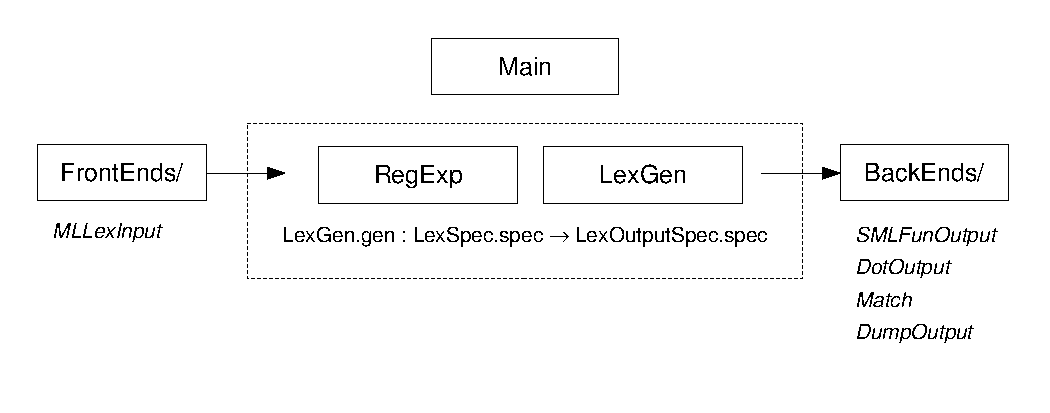
\includegraphics[scale=0.8]{impl-pic.pdf}
\fi
\end{center}
\caption{\ulex{} organization}
\end{figure}

\section{\nm{RegExp}}\label{sec:reg-exp}

In \ulex{}, REs are captured by the abstract type \nm{RegExp.re}.  Introduction
is provided by various ``smart constructors'' (\nm{mkSym}, \nm{mkClosure},
$\dots$), and elimination is provided by the derivatives algorithm.  The
signature for the \rm{RegExp} module is shown below:

\begin{verbatim}
signature REG_EXP =
  sig

    structure Sym : INTERVAL_DOMAIN
    structure SymSet : INTERVAL_SET

    type symbol
    type sym_set
    type re

    val any       : re  (* wildcard *)
    val none      : re  (* EMPTY language *)
    val epsilon   : re  (* the nil character (of length 0) *)

    val mkSym     : symbol -> re
    val mkSymSet  : sym_set -> re

    val mkOr      : re * re -> re
    val mkAnd     : re * re -> re
    val mkXor     : re * re -> re
    val mkNot     : re -> re
    val mkConcat  : re * re -> re
    val mkClosure : re -> re
    val mkOpt     : re -> re
    val mkRep     : re * int * int -> re
    val mkAtLeast : re * int -> re

    val isNone    : re -> bool
    val nullable  : re -> bool
    val derivative : symbol -> re -> re
    val derivatives : re Vector.vector ->
                      ((re Vector.vector) * sym_set) list

    val symToString : symbol -> string
    val toString  : re -> string
    val compare   : re * re -> order

  end
\end{verbatim}

The included structure \nm{SymSet} provides symbol interval sets, which are
ideal when working with dense sets such as unicode character classes.  Interval
set operations (\nm{union}, \nm{complement}, $\dots$) are used extensively;
documentation for the interval set library is available with the SML/NJ
distribution.

Recall that, in using RE derivatives for DFA construction, it is
important to aggresively identify when two REs generate the same
language so that they may be merged to a single state in the automaton.
\nm{RegExp} canonicalizes REs, which is why its \nm{re} type is abstract.
Canonicalization is performed using a lexicographic ordering on REs given by the
\nm{compare} function.  The comparison is lexicographic in the sense that it
first examines the top-level operation of the two REs, and only does more
comparisons if that operation is the same.  We represent REs as follows:
\begin{verbatim}
    datatype re
      = Epsilon
      | Any
      | None
      | SymSet of sym_set
      | Concat of re list
      | Closure of re
      | Op of (rator * re list)
      | Not of re
    and rator = OR | AND | XOR
\end{verbatim}
For the \nm{Op} constructor, which is used for three different commutative
operations, the sub-REs are to be listed in canonical order. The \nm{compare}
function itself will expect that this is the case, and since only smart
constructors can be used to construct REs, the invariant will always hold.

Smart constructors do additional canonicalization beyond ordering.  For
example, \nm{mkNot (mkNot (none))} will be canonicalized
to the same representation as \nm{none}.  Several similar RE equalities
are detected and used.  Also, the smart constructors attempt to push the RE
reprsentation as much toward symbol sets as possible, replacing boolean
operations at the RE level with a single resulting symbol set when possible.
For example, suppose that \nm{AM} held the symbol set for $[A-M]$, \nm{HZ} the
set for $[H-Z]$, and \nm{AZ} the set for $[A-Z]$. Then we would have
\[
\texttt{compare (mkSymSet AZ, mkOr (mkSymSet AM, mkSymSet HZ)) = EQUAL}
\]
The hope is that the cumulative effect of such canonicalization will keep the
generated DFA close to minimal size.

The \nm{derivatve} function constructs a canonicalized derivative for a given
RE with respect to a given symbol; it is a transcription of the algorithm
described in section~\ref{sec:derivatives}.

In general, we will be interested in the derivatives of a vector of REs
(representing the rules in a lexer specification) with respect to \emph{every}
symbol in the alphabet.  As section~\ref{sec:factorings} explains, the unicode
alphabet is too large for us to literally test the derivative at each symbol. 
The \nm{derivatives} function will take a vector of REs and return a list of
\nm{re~Vector.vector~*~sym\_set} \emph{pairs}.  In fact, \nm{derivatives}
is just an implementation of the factor and compress algorithm given
in~\ref{sec:factorings}.  Each pair in the result list represents an arrow
transitioning out of the current state (which corresponds to the input RE
vector) to a new state (the output RE vector) on a given set of symbols (the
output symbol set).  Thus the labor of DFA construction is split between the
\nm{RegExp} module, which computes derivatives (and hence transitions) and
\nm{LexGen}, which actually constructs the DFA graph.

\section{\nm{LexSpec} and \nm{LexOutputSpec}}

Before describing DFA generation, we briefly discuss the relevant input and
output data structures.  The \nm{LexSpec} module has data constructors and
functions relevant to \eg the ML-Lex input specification format, as shown in
Figure~\ref{fig:lex-spec}

\begin{figure}
\begin{verbatim}
    type action = string
    type rule_spec = AtomSet.set option * RegExp.re
    type rule = rule_spec * action

    datatype spec = Spec of {
        decls : string,
        conf : config,
        rules : rule list
      }
\end{verbatim}
\caption{A fragment of \nm{LexSpec}}\label{fig:lex-spec}
\end{figure}

Actions, at least in the present implementation, are just raw strings.  A
\nm{rule} consists of a rule specification and an associated action.  The
optional atom set included with a rule spec represents the start states
to which that rule applies (with \nm{NONE} meaning, strangely enough, all start
states).  With these definitions, a lexer specification is just a list of
rules, some declarations (a raw string containing code) and some miscellaneous
configuration data.

\begin{figure}
\begin{verbatim}
    datatype dfa_state
      = State of {
          id : int,
          label : RegExp.re Vector.vector,
          final : int list,
          next :  (RegExp.sym_set * dfa_state) list ref
        }

    datatype machine = Machine of {
        label : string,
        rules : (RegExp.re * int) vector,
        states : dfa_state list
      }

    type action = string

    datatype spec = Spec of {
        actions : action vector,
        machines : machine list,
        ...  (* configuration data *)
      }
\end{verbatim}
\caption{A fragment of \nm{LexOutputSpec}}\label{fig:lex-output-spec}
\end{figure}

As Figure~\ref{fig:lex-output-spec} illustrates, the output of DFA generation is
\emph{not} a DFA, but a collection of DFAs along with a vector of actions. 
Each \nm{machine} represents a start state for the lexer; that is, each start
state has its own automaton.  However, since start states may use the same
actions, we separate out the actions into a vector so that they are only
emitted once.

A \nm{machine} includes a label, which is just the name of the start state, as
well as the rules relevant to that machine, which are paired with an index to
the associated action in the action vector.  The DFA itself is a list of
states, with the head of the list being $q_0$.  A state, in turn, is labeled by
a vector of REs (with the same length as the \nm{rules} vector in the machine).
 Since a given DFA state may be an accepting state for more than one rule, we
store a \emph{list} of rule indices for the \nm{final} flag.  On a match, the
action for the lowest-index rule is executed first, but that action may use
\nm{REJECT()}, in which case it may be necessary to jump to the action for the
next rule index given in the \nm{final} list.

\section{\nm{LexGen}}\label{sec:lex-gen}

\nm{LexGen} is a very simple module with a single accessible function:
\begin{center}
\nm{gen : LexSpec.spec -> LexOutputSpec.spec}
\end{center}

The first task of the \nm{gen} function is to collate the actions and start
states.  The actions from the input spec are separated from their rules into a
vector.  Afterwards, \nm{gen} iterates over the specified start states,
collecting the rules for each start state and using the \nm{mkDFA} function to
generate a machine for each.

\nm{mkDFA} performs a straightforward imperative DFA construction, using
the \nm{derivatives} function from \nm{RegExp} to compute the transitions out of
each node. A map of RE vectors to DFA nodes is maintained (using
\nm{Vector.collate RegExp.compare} for ordering); this map is used to recognize
when a new out-edge is going to an existing DFA node.  Finally, any transition
to a vector of REs which all generate the empty language is an error transition
(that is, the derivatives for the given transition symbol set all indicate a
non-match).

\section{Front ends}

At the moment, only one front end is available: the ML-Lex specification
format.  Eventually \ulex{} will have its own format.

The ML-Lex front end is fairly straightforward: it uses ML-Yacc to do the
parsing, and can use either ML-Lex or \ulex{} to do the lexing.  The
distribution includes a lexer that was generated from \ulex{} to serve as a
bootstrap.

\section{Back ends}

One exciting aspect of \ulex{} is the ability to easily add back ends.  The
following back ends are currently included in the distribution.

\paragraph{SML control-flow lexer generation}

The most important back end is code generation for SML.  At present, there is a
single code generation strategy: build a lexer using control-flow (\ie
if statements and tail-calls) to match the input.  If the control-flow strategy
turns out to be inadequate, it would be fairly easy to add a code
generator for table-based lexing.

Code generation is performed by expanding stubs in a template SML file.  The
template contains code for dealing with streams and setting up the lexer in the
appropriate way.  Input is read from functional strings, which allow for
the arbitrary lookahead needed for maximal-munch.  These streams also track
the current file position and line number.

A helper module, \nm{ML}, contains a representation for a good portion of the
Standard ML expression langauge, and support for pretty-printing such
expressions.

The generated code includes user actions and the DFA for each start state.
 Within each start state there is one \emph{state function} per DFA node.  Each
state function will examine the next character of input and perform a series of
if-tests to determine the correct transition.  The if-tests perform a
hard-coded binary search over the symbol set intervals for the transitions.

The lexer stores a reference cell for the current functional stream.  Each time
the lexer accepts a token, the cell is updated.  \nm{yytext} is generated (only
when needed) by ``subtracting'' the new stream from the one stored in the
reference cell before updating it.  Subtraction simply rescans the appropriate
number of characters from the stored stream, which should still have the string
in its buffer.

One subtlety is handling calls to \nm{REJECT()}.  Since such calls are fairly
rare, we want to avoid tracking the information \nm{REJECT} needs if it won't
be used.  \nm{REJECT} information consists of (in essence) a list of all the
previous matches.  A previous match could occur on the same DFA state if
multiple REs matched the input at that state; otherwise, the previous match is
a prefix of the \nm{REJECT}ed match.  Whenever a transition is made, the
appropriate previous match information is passed up to the next state. 
However, if the current state is an accepting state that does not use
\nm{REJECT}, then the history is \emph{truncated} at the \nm{REJECT}-free
point, since it could never be used.  This determination is made statically and
is hard-coded into the generated SML lexer.

\paragraph{Graphviz}

The Graphviz toolkit provides easy graph visualization using a very simple
graph description format.  We utilize the DOT format.  The Graphviz backend
will write one DOT file for each start state, showing all nodes for that start
state's DFA, along with labeled transitions.  See \texttt{www.graphviz.org} for
details on the DOT format.

\paragraph{Text dump}

If Graphviz is not available or a more detailed summary is desired, the
\nm{DumpOutput} module can be used to print to standard out every DFA state,
labeled by its RE vector, along with out-edges, for every start state in the
lexer.

\paragraph{Interactive matching}

Finally, a simple interactive back end is available.  Interactive matching
allows a user to enter arbitrary strings and find out (1) if they matched and
(2) what RE matched them.  The code for interactive matching is quite simple.

\section{\nm{Main}}

The \nm{Main} module is the driver for \ulex{}: it is responsible for processing
command-line arguments and hooking up the appropriate front and back ends. 
Since it is very simple, it gives a nice overview of the system and is a good
place to look first in trying to undertand the code.